\documentclass{beamer}
\mode<presentation>{
\usetheme{Madrid}
}
\usepackage{graphicx}
\usepackage{booktabs}
\usepackage{multicol}

%--------------------------------------------------
%	TITLE PAGE
%--------------------------------------------------
\title[Citation Network Proposal]{Citation Network Proposal}

\author[Group 2 - ADB Course]{Group 2\\MITIU14005 - Nguyen Hoang Minh \\ MITIU14006 - Chiem Thach Phat}

\institute[HCMIU]{Ho Chi Minh City, International University}

\date{\today}

%--------------------------------------------------
\begin{document}
%--------------------------------------------------
\begin{frame}
\titlepage
\end{frame}

\begin{frame}
\frametitle{Table of Contents}
\tableofcontents
\end{frame}
%--------------------------------------------------
\section{Introduction}
%--------------------------------------------------
\begin{frame}
\frametitle{Table of Contents}
\tableofcontents[currentsection]
\end{frame}

\begin{frame}
\frametitle{Motivation}
The world needs a citation network for patents to:
\begin{itemize}
\item Analyzing trending in field
\item Looking up for the existence of similar patents
\item Finding who invents most patents
\end{itemize}
\end{frame}

%--------------------------------------------------
\section{Implementation}
%--------------------------------------------------
\begin{frame}
\frametitle{Table of Contents}
\tableofcontents[currentsection]
\end{frame}

\begin{frame}
\frametitle{Analyzing the Scenario}
We would like to build a citation network for patents with these constraints:
\begin{itemize}
\item Able to store and analyze patents from USPTO bulk data.
\item A patent contains: an unique Publication Number, Publication Type, Application Number, Publication Date, Filling Date, Priority Date, Fee Status, Title, Length of Grant, Classification and some of its contents include Abstract, Images, Description and Claims
\item A Patent may or may not cite/be cited other patents
\item A Patent must be invented/applied/examined by or assigned for at least one Inventor, Applicant, Examiner or Assignee
\item Inventor, Applicant, Examiner and Assignee are identified by first name, last name, city and country
\end{itemize}
\end{frame}

\begin{frame}
\frametitle{Conceptual Model}
Based on the scenario, we have designed this conceptual model.
\begin{center}
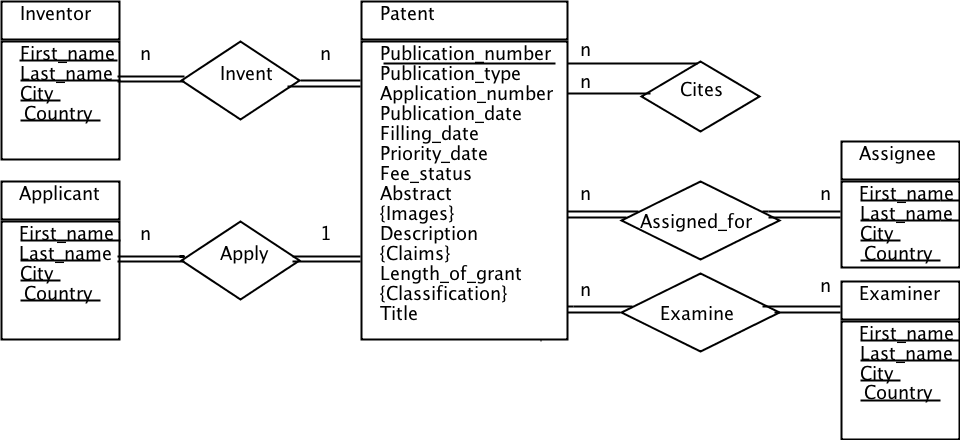
\includegraphics[height=2in]{full_er.png}
\end{center}
\end{frame}

\begin{frame}
\frametitle{Implemented Conceptual Model}
Due to time constraint, we use this conceptual model to implement the citation network.
\begin{center}
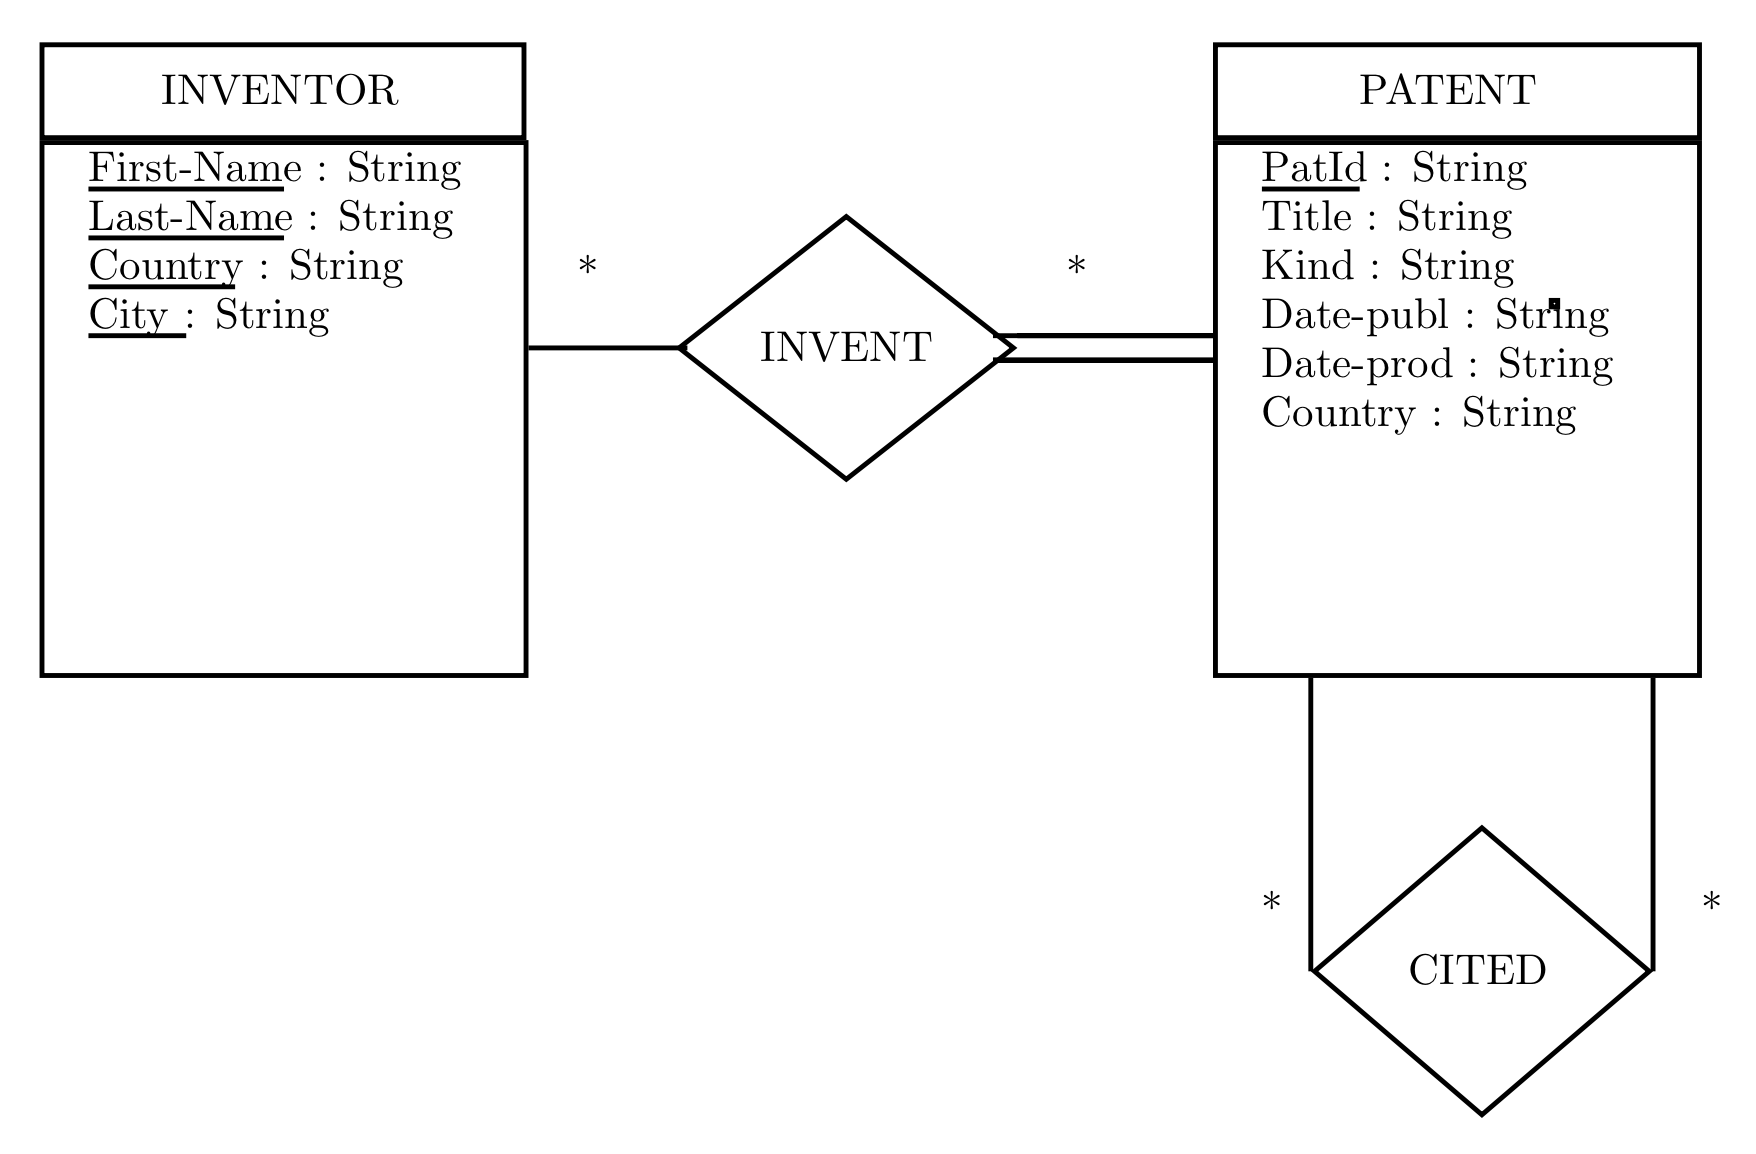
\includegraphics[height=2in]{implemented_er.png}
\end{center}
\end{frame}

\begin{frame}
\frametitle{Logical Model - Neo4j}
Neo4j use the concept of \textbf{Nodes}, \textbf{Properties} and \textbf{Relationships} as shown in the picture below, where:
\begin{itemize}
\item Nodes: PATENT, INVENTOR
\item Properties: Nodes and Relationships attributes, such as Patent\_No or Cited\_date
\item Relationships: CITEDBY, INVENT
\end{itemize}
\begin{center}
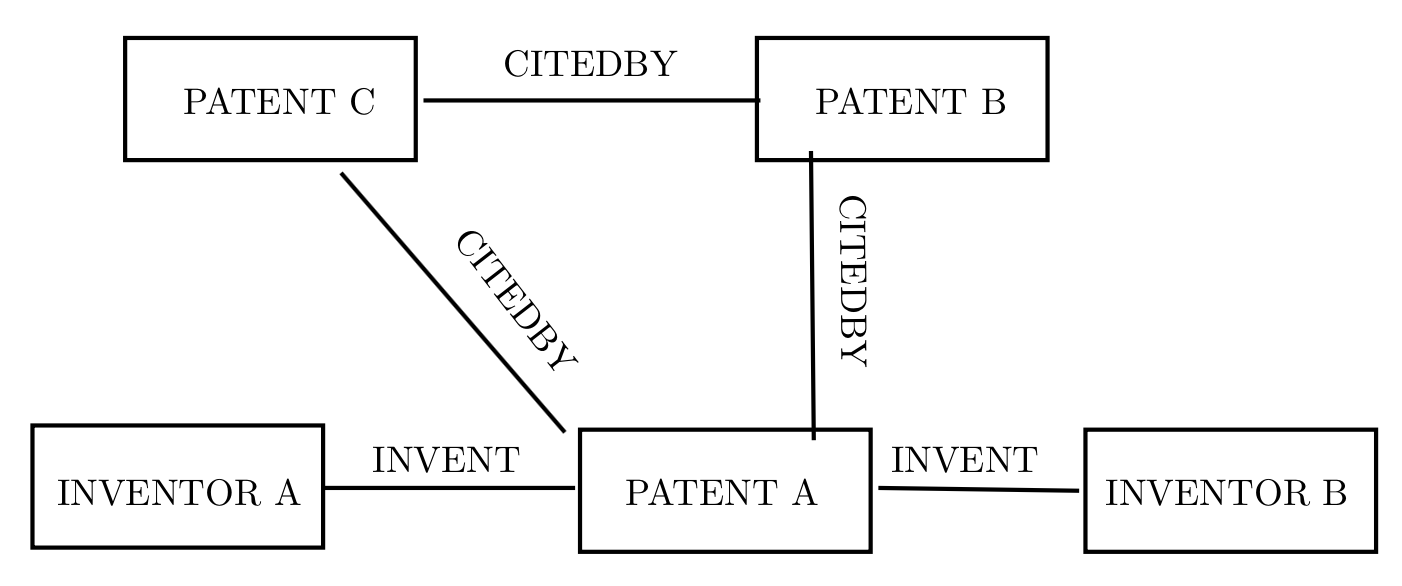
\includegraphics[height=1.8in]{neo4j.png}
\end{center}
\end{frame}

\begin{frame}
\frametitle{Logical Model - Neo4j (Cont.)}
Pros:
\begin{itemize}
\item Can cope with complex relationship
\item Offers more accurate ways to determine the relationship between each entity
\end{itemize}
Cons:
\begin{itemize}
\item Slow with complex search
\item Built-in Web Server is not supported for visualizing more than 1000 rows
\end{itemize}
\end{frame}

\begin{frame}
\frametitle{Logical Model - MongoDB}
While Neo4j stores data in Nodes, Properties and Relationships, \textbf{MongoDB stores data as a BSON file}.
\begin{center}
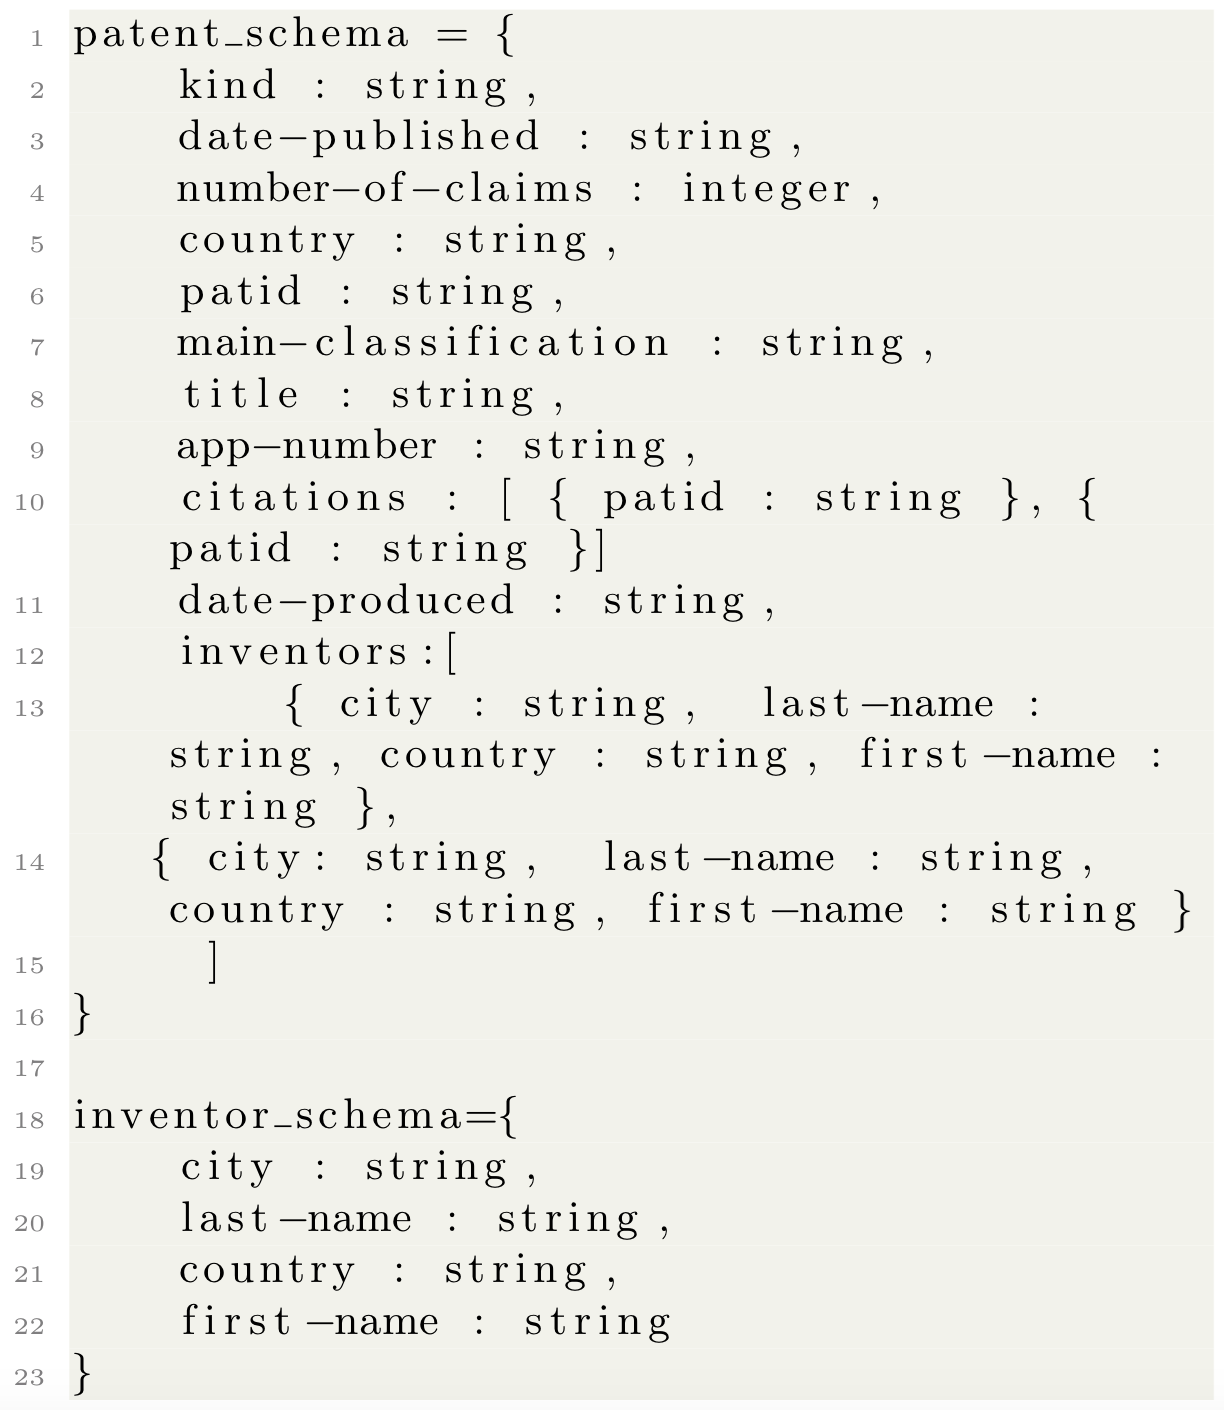
\includegraphics[height=2.6in]{mongodb.png}
\end{center}
\end{frame}

\begin{frame}
\frametitle{Logical Model - MongoDB (Cont.)}
Pros:
\begin{itemize}
\item Documents (i.e. objects) can be defined with native data types that can be seen in many programming languages. E.x: Date, String, Integer
\item Embedded documents and arrays reduce need for expensive joins
\item Dynamic schema supports fluent polymorphism
\end{itemize}
Cons:
\begin{itemize}
\item Does not support relationship
\end{itemize}
\end{frame}

\begin{frame}
\frametitle{CINAS Structure}
Our CINAS will follow the structure below, starts from the Patent XML File and ends at \textbf{Neo4J DB and MongoDB as our data storages}.
\begin{center}
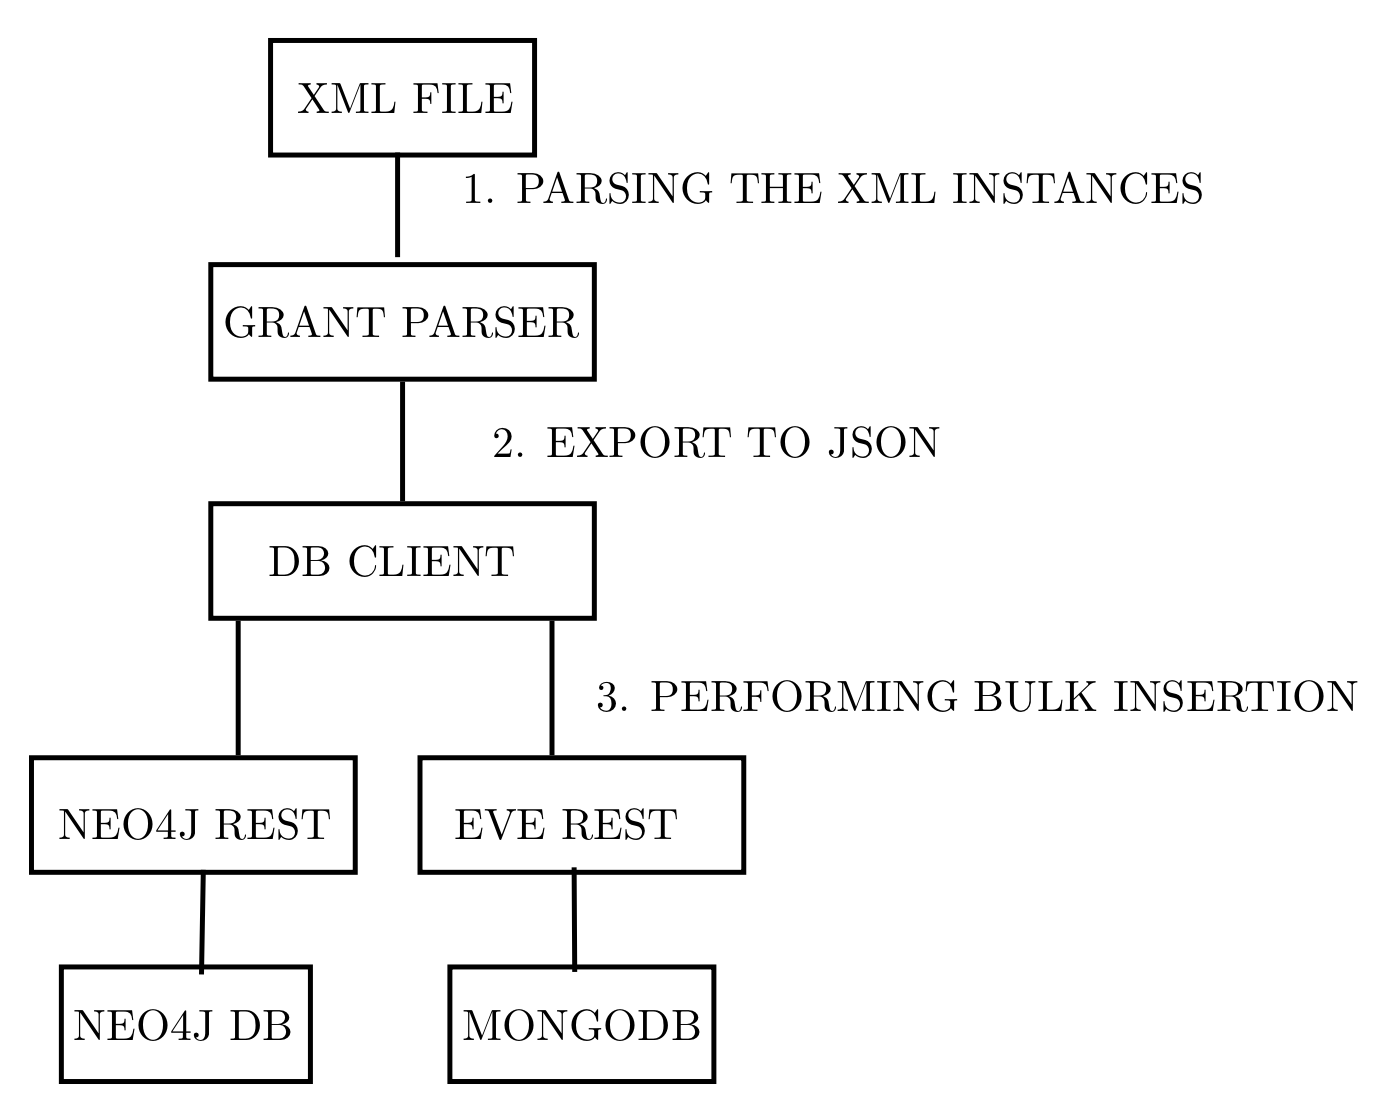
\includegraphics[height=2in]{cinas.png}
\end{center}
\end{frame}

\begin{frame}
\frametitle{Grant Parser Module}
Due to the enormous size of the Patent Bulk Download File, we will use \textbf{SAX method} instead of DOM method to \textbf{process the XML file}.\\~\\
Pseudocode for \textbf{Grant Parser Module}:
\begin{enumerate}
\item Load XML file and break it down into separated XML instances
\item Parse each XML instance into patent handler. For each tag with nested tags, enable stack to store adjacent data
\item Tags that are explicitly defines in ignore list will be left out during parsing. Upon completion, reset the patent handler for new instance
\item Finally, an option to export the entire file to JSON format is available if chosen
\end{enumerate}
\end{frame}

\begin{frame}
\frametitle{DB Client Module}
We chose to deploy REST services in communication with our backends instead of OM to provide more scalable solution as we just use HTTP response and request.\\~\\
\textbf{DB Client Class Diagram:}\\
\begin{center}
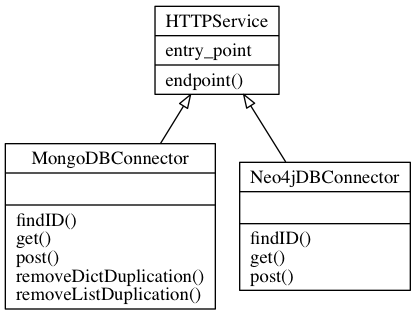
\includegraphics[height=2in]{dbclient.png}
\end{center}
\end{frame}

\begin{frame}
\frametitle{DB Client Module (Cont.)}
Pseudocode for \textbf{POST in MongoDBConnector}:
\begin{enumerate}
\item Load all data from JSON file
\item Construct list of citations from group of patent
\item Validate uniqueness within the list
\item Appending statements into query. Then, perform 1st POST these citations
\item If the uniqueness is violated, the response code from EVE server will determine the next step. If error response with duplicates found, remove it from the list and resend it again
\item Finally, perform an overwrite PUT for any individual patent. This step must be linearly execute to guarantee that all the dummy patents, which are created using citations, will be updated with information
\end{enumerate}
\end{frame}

\begin{frame}
\frametitle{DB Client Module (Cont.)}
POST in Neo4j is more simpler because it has an overwrite operation called \textbf{``MERGE''}, which \textbf{automatically detect duplication and merge together or create new one}.\\~\\
Pseudocode for \textbf{POST in Neo4jDBConnector}:
\begin{enumerate}
\item Load all data from JSON file
\item Construct list of citations from group of patent
\item Appending statements into query. Then, perform POST these citations
\item Finally, we perform another POST for list of patents
\end{enumerate}
\end{frame}

\begin{frame}
\frametitle{Citation Network Visualization}
For Citation Network Visualization, we wrote \textbf{generate\_csv} to automate the process:
\begin{enumerate}
\item Assuming that Neo4J is populated using \textbf{DB Client}
\item Run \textbf{generate\_csv} will results in 2 csv files : nodes.csv and links.csv
\item Use GEPHI to load these files and visualize the data
\end{enumerate}
\begin{center}
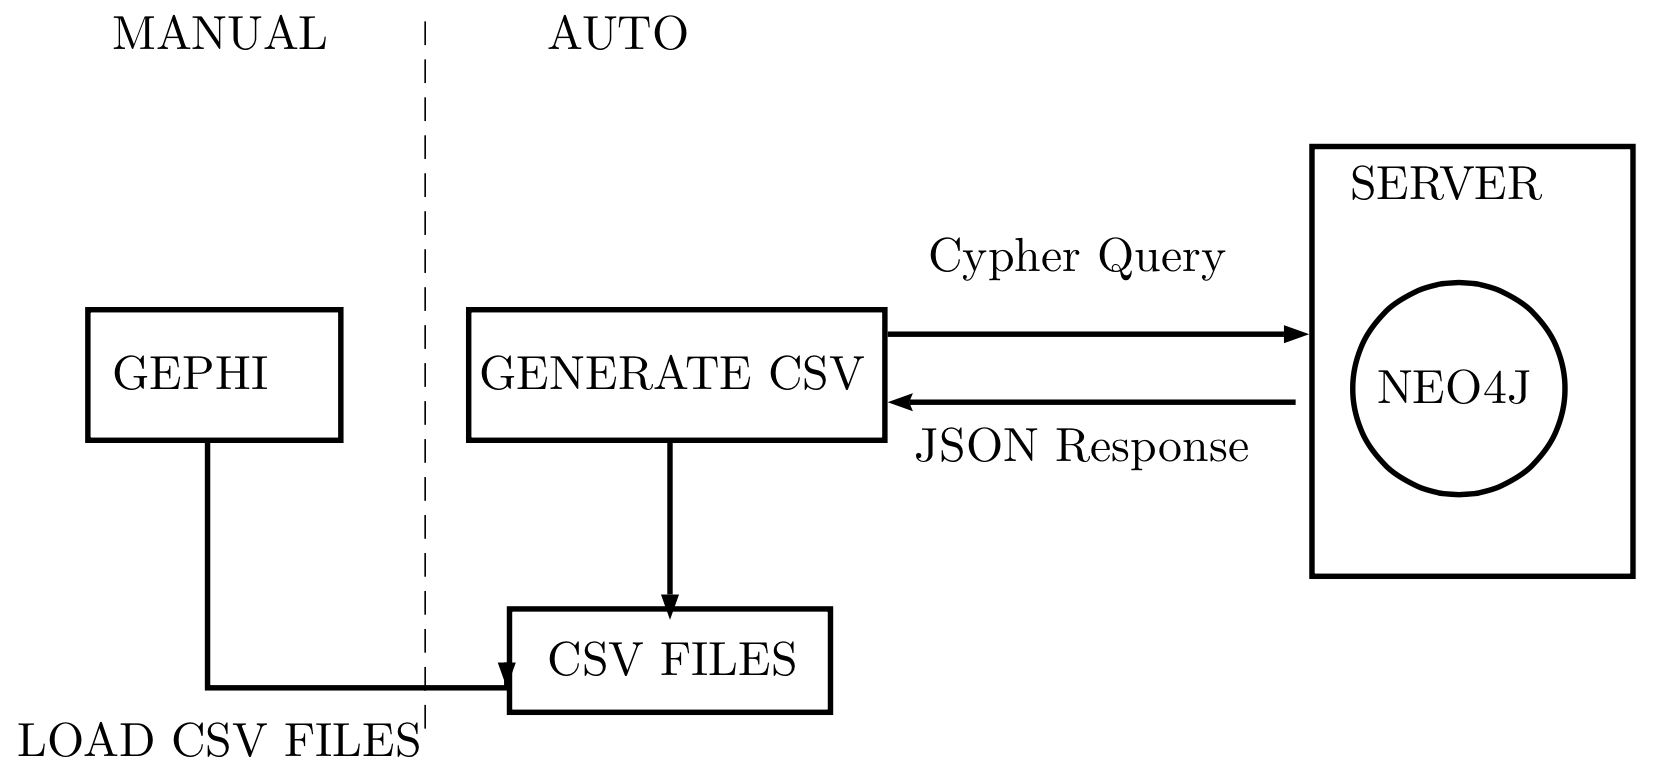
\includegraphics[height=2in]{gephi.png}
\end{center}
\end{frame}

%--------------------------------------------------
\section{Results}
%--------------------------------------------------
\begin{frame}
\frametitle{Table of Contents}
\tableofcontents[currentsection]
\end{frame}

\begin{frame}
\frametitle{Results}
Processed patents:
\begin{table}[htd]
\begin{tabular}{|c|c|l|} \hline
 &Number of Documents\\ \hline
 Duplicated Citations&347 \\ \hline
Patents&3000 \\ \hline
Citations&106996 \\ \hline
Total & 110343\\ \hline
\end{tabular}
\end{table}
\end{frame}

\begin{frame}
\frametitle{Results (Cont.)}
The figure illustrates Patent Classification in October 2014.\\~\\
The MISCELLANEOUS (\textbf{D99}) industry were blossomed in October 2014
\begin{center}
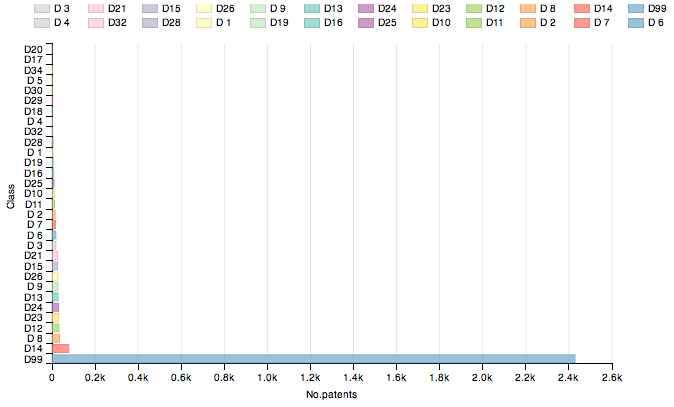
\includegraphics[height=2in]{rplot-classification.png}
\end{center}
\end{frame}

\begin{frame}
\frametitle{Citation Network}
The figure shows a citation network with 500 patents in the database.\\~\\
D0714930, D0714929 and D0714813 were the most popular in rank based on connected components.
\begin{center}
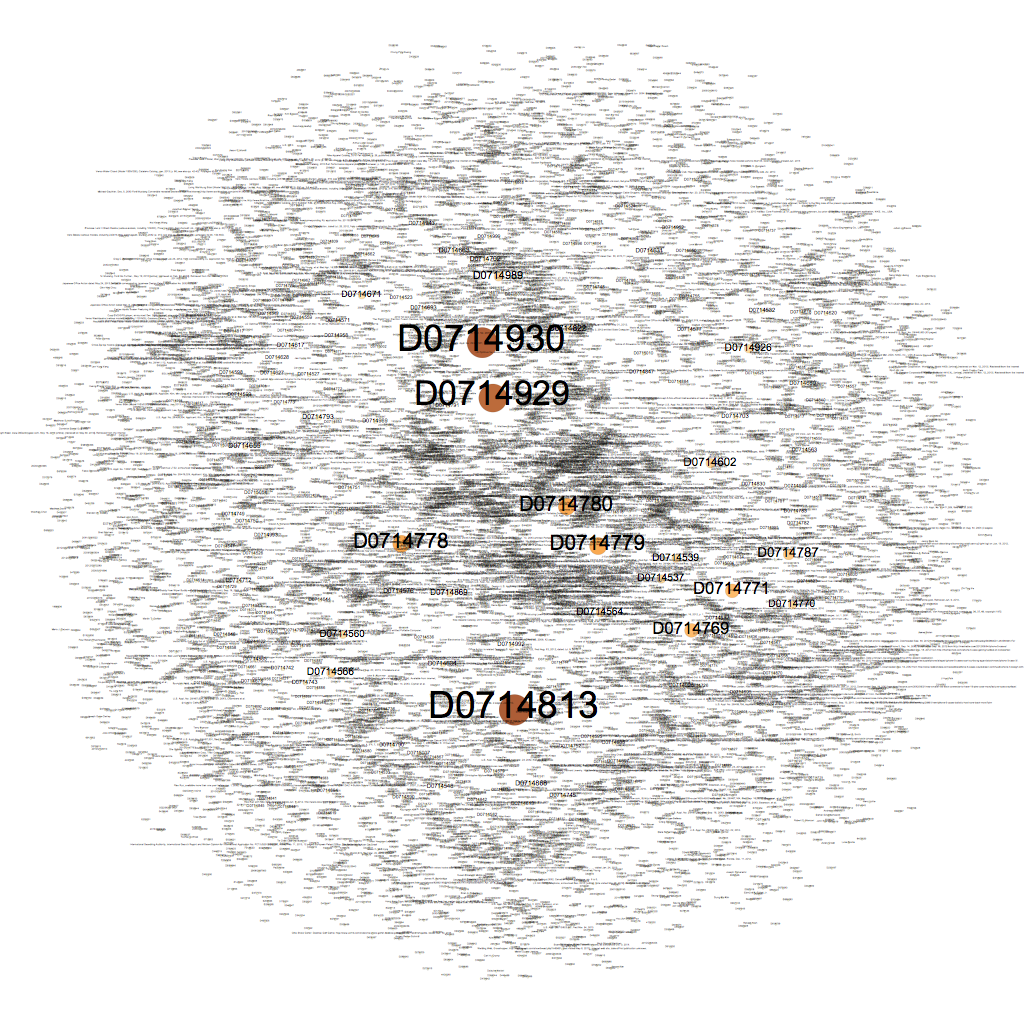
\includegraphics[height=2.6in]{citation-label.png}
\end{center}
\end{frame}

\begin{frame}
\frametitle{Inventors Maps}
To measure the activity of inventors community, we classify them based on their regions.\\~\\
Most of inventors come from North America. Furthermore, US patents industry also attracts the numerous inventors from different parts of the world, including Asian and Australian.
\begin{center}
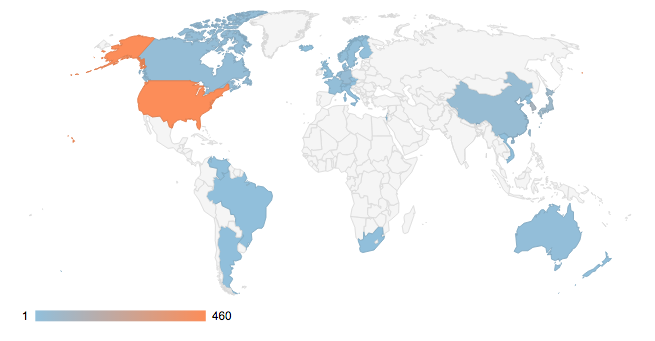
\includegraphics[height=2in]{inventor-map.png}
\end{center}
\end{frame}

\begin{frame}
\frametitle{Benchmark Neo4j and MongoDB}
We perform the time measurements on 500 patents with total of 12016 citations.\\
\begin{multicols}{2}
Results:
\begin{itemize}
\item \textbf{DOM} parser is \textbf{faster} than \textbf{SAX}
\item \textbf{Object-Mapping} is \textbf{faster} than \textbf{REST}, but \textbf{REST} is \textbf{easier to extend} than Object-Mapping
\item Populate data in \textbf{MongoDB} is \textbf{faster} than \textbf{Neo4j}, but the drawback is MongoDB client has to implement references between documents
\end{itemize}
\columnbreak
\begin{center}
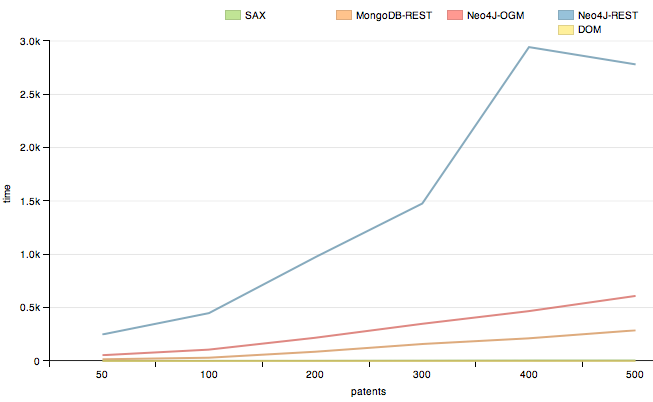
\includegraphics[width=0.5\textwidth]{line.png}
\end{center}
\end{multicols}
\end{frame}
%--------------------------------------------------
\section{Lesson Learned}
%--------------------------------------------------
\begin{frame}
\frametitle{Table of Contents}
\tableofcontents[currentsection]
\end{frame}

\begin{frame}
\frametitle{Lesson}
\begin{itemize}
\item Choice of technology
	\begin{itemize}
	\item Analyzing citation network with Neo4J is much simpler than MongoDB \& RDBMS.
	\item Neo4J web server only visualizes up to 1000 rows.
	\item Object-Mapping is faster and easier to use than REST. However, REST is more suitable for scalable system that involves different languages \& platforms that communicate via JSON. 
	\item Drawbacks of Normalization in RDBMS since it can't fully represent the natural language . Hence, we chose MongoDB to store data.
	\end{itemize}
\item Patent
	\begin{itemize}
		\item It's inevitable that patent can help identify the trend of inventions in one country's industry.
		\item Further analysis may take into account the backward citation and forward citation to identify the trend on time basis.
	\end{itemize}
\end{itemize}
\end{frame}
%--------------------------------------------------
\section{Future works}
%--------------------------------------------------
\begin{frame}
\frametitle{Table of Contents}
\tableofcontents[currentsection]
\end{frame}

\begin{frame}
\frametitle{Future Works}
\begin{itemize}
\item Divide patent data into different databases instead of storing the whole file into one particular back-end
\item Propose a refined structure for storing and querying patent data across multiple database systems
\item Provide an end-user services that would transform natural language into our CINAS's language, process the queries, determine the keywords and then pass it to the suitable database system
\item Final goals:
\begin{enumerate}
\item Take advantages of multiple database systems
\item Reduce the query costs
\item Enhance end-users experience with patent data
\end{enumerate}
\end{itemize}
\end{frame}

\begin{frame}
\frametitle{References}
[1] ``Transitioning from Relational Databases to MongoDB - Data Models'' B. Reinero, http://blog.mongodb.org/post/72874267152/transitioning-from-relational-databases-to-mongodb, Jan 2014\par
[2] ``USPTO Patents Database Construction" I. Torvik, D. Dubin and Q.Liu, http://abel.lis.illinois.edu/UPDC/USPTOPatentsDatabaseConstruction.pdf, August 2012\par
[3] ``Construction of Japanese Patent Database for Research on Japanese patenting activities" A. Goto, K. Motohashi, http://www.iip.or.jp/e/images/paper.pdf
\end{frame}

\begin{frame}{Thank You}
\begin{center}
Thank you for your listening!
\end{center}
\end{frame}

\end{document}